\subsection{OTFS Simulation Flow}

The previous sections have described the baseline OTFS system from the transmitter, channel, receiver, input-output model, and detector perspectives. This section connects these individual processing blocks into the end-to-end simulation flow used for BER evaluation. The purpose is not to introduce a new theoretical model, but to clarify how the baseline OTFS chain is executed in MATLAB before it is used as a reference system in the performance evaluation chapter.

In the simulation framework, the baseline OTFS system is evaluated through an end-to-end Monte Carlo loop. For each value of \(E_b/N_0\), the simulator generates random information bits, maps them into QAM symbols, places the symbols on the delay-Doppler grid, applies OTFS modulation, passes the transmitted signal through the delay-Doppler multipath channel, performs OTFS demodulation, detects the transmitted symbols using the MP detector, and finally computes the BER by comparing the detected bits with the transmitted bits.

\begin{figure}[H]
    \centering
    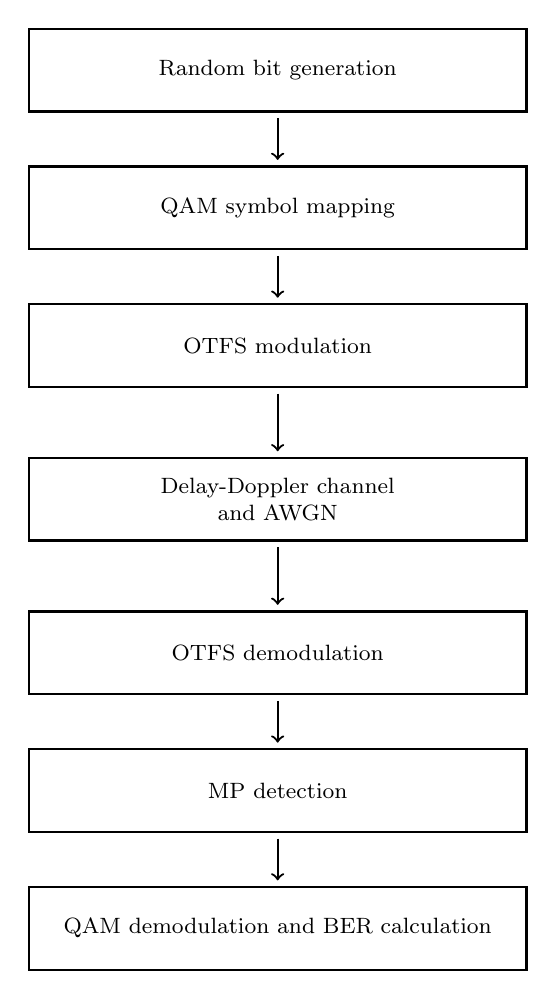
\begin{tikzpicture}[
        block/.style={
            rectangle,
            draw,
            thick,
            align=center,
            text width=5.9cm,
            minimum height=1.05cm,
            font=\footnotesize,
            inner sep=6pt
        },
        arrow/.style={
            ->,
            thick,
            shorten >=2pt,
            shorten <=2pt
        }
    ]

        \node[block] (bits) at (0,0) {Random bit generation};
        \node[block] (qam) at (0,-1.75) {QAM symbol mapping};
        \node[block] (mod) at (0,-3.50) {OTFS modulation};
        \node[block] (chan) at (0,-5.45) {Delay-Doppler channel\\and AWGN};
        \node[block] (demod) at (0,-7.40) {OTFS demodulation};
        \node[block] (mp) at (0,-9.15) {MP detection};
        \node[block] (ber) at (0,-10.90) {QAM demodulation and BER calculation};

        \draw[arrow] (bits.south) -- (qam.north);
        \draw[arrow] (qam.south) -- (mod.north);
        \draw[arrow] (mod.south) -- (chan.north);
        \draw[arrow] (chan.south) -- (demod.north);
        \draw[arrow] (demod.south) -- (mp.north);
        \draw[arrow] (mp.south) -- (ber.north);

    \end{tikzpicture}
    \caption{Baseline OTFS simulation flow used for BER evaluation}
    \label{fig:baseline_otfs_simulation_flow}
\end{figure}

Figure~\ref{fig:baseline_otfs_simulation_flow} summarizes the simulation flow. The first stage creates an equiprobable binary information sequence
\begin{equation}
    \mathbf{b}
    \in
    \{0,1\}^{N_{\mathrm{bits}}},
    \qquad
    \Pr(b_i=0)=\Pr(b_i=1)=\frac{1}{2}.
    \label{eq:baseline_random_bits}
\end{equation}
The generated bits are then grouped according to the QAM order and mapped to complex QAM symbols. For the baseline OTFS case, all delay-Doppler positions carry QAM symbols, because no index modulation is applied at this stage.

The mapped QAM symbols are reshaped into the \(N\times M\) delay-Doppler grid and processed by the OTFS transmitter described in Section 3.2. The output is a time-domain transmit vector. A channel realization is then generated by specifying the number of paths, delay taps, Doppler taps, and complex channel coefficients. The transmitted signal is passed through this time-varying multipath channel and corrupted by AWGN.

At the receiver, OTFS demodulation transforms the received time-domain signal back to the delay-Doppler observation grid. The MP detector then estimates the transmitted symbols from this observation using the sparse delay-Doppler channel structure. The estimated QAM symbols are demodulated back into bits, and the BER is computed as
\begin{equation}
    \mathrm{BER}
    =
    \frac{N_{\mathrm{err}}}{N_{\mathrm{bits}}},
\end{equation}
where \(N_{\mathrm{err}}\) is the number of incorrectly detected bits and \(N_{\mathrm{bits}}\) is the total number of transmitted bits over the simulated frames.

The baseline OTFS simulation also supports adaptive stopping in the Monte Carlo loop. If adaptive simulation is enabled, the number of frames at a given \(E_b/N_0\) point can stop early after a minimum number of frames and a target number of bit errors have been reached. This keeps the simulation practical while still collecting enough errors for BER estimation. If adaptive simulation is not enabled, the simulator uses the fixed number of frames specified in the configuration.

The baseline OTFS simulation outputs include the accumulated bit errors, the number of frames used at each SNR point, and the resulting BER vector. These outputs are later combined with the OFDM, OTFS-IM, and pattern-selection results in the main experiment runner. Therefore, the baseline OTFS flow provides the reference BER curve against which the proposed OTFS-IM schemes are evaluated in Chapter 5.
